% Begin the document and set up the style of the document
\documentclass[a4paper]{article}

% Install the required packages for the document 
\usepackage{envmath}
\usepackage{esvect}
\usepackage{graphicx}
\usepackage{gensymb}
\usepackage{tikz}
\usepackage[mathcal]{euscript}
\usepackage{geometry}
\usepackage{enumitem}
\usepackage{mathtools}
\usepackage{graphicx}
\usepackage{amsmath}
\usepackage{amscd}
\usepackage{amssymb}
\usepackage{amsfonts}
\usepackage{harpoon}
\usepackage{pgf}
\usepackage{tikz}
\usepackage{mathrsfs}
\usepackage{asyalign}
\usepackage{physics}
\usepackage{enumitem}
\usepackage{xhfill}
\usepackage{accents}
\usepackage{cite}
\usepackage{url}
\usepackage[tableposition=top]{caption}
\usepackage{ifthen}
\usepackage[utf8]{inputenc}
\usepackage{tikz-3dplot}
\usetikzlibrary{patterns}
\usetikzlibrary{arrows}

% Page and style settings
\parskip=8pt
\parindent=0pt
% Right margin
\textwidth=6.25in
% Left margin
\oddsidemargin=0pt
\evensidemargin=0pt
% Bottom margin
\textheight=10in
% Top margin
\topmargin=-0.75in
\baselineskip=11pt
% end of page and other style settings

\renewcommand{\familydefault}{\sfdefault}

\newcommand{\indep}{\mathrel{\text{\scalebox{1.07}{$\perp\mkern-10mu\perp$}}}}

% Begin the text of the document
\begin{document}

% Begin the Title Page
\begin{titlepage}

\newcommand{\HRule}{\rule{\linewidth}{0.5mm}} % Defines a new command for the horizontal lines, change thickness here

\center % Center everything on the page
 
\textsc{\LARGE University of Sydney}\\[1.5cm] % Name of your university/college
\textsc{\Large MATH 1907}\\[0.5cm] % Major heading such as course name
\textsc{\large SSP}\\[0.5cm] % Minor heading such as course title

\HRule \\[0.4cm]
{ \huge \bfseries Assignment 3 - Statistics}\\[0.4cm] % Title of your document
\HRule \\[1.5cm]

\begin{minipage}{0.4\textwidth}
\begin{flushleft} \large
\emph{Author:}
Keegan Gyoery % Your name
\\
\emph{SID:}
470413467
\end{flushleft}
\end{minipage}
~
\begin{minipage}{0.4\textwidth}
\begin{flushright} \large
\emph{Lecturer:} 
Rachel Wang % Tutor's Name
\\
\emph{Seminar:}
New Law Annexe SR 346
Tuesday 4pm
\end{flushright}
\end{minipage}\\[4cm]

{\today}\\[3cm] % Date, change the \today to a set date if you want to be precise

\vfill % Fill the rest of the page with whitespace

\end{titlepage}

\pagenumbering{arabic}

\begin{enumerate}[label=\textbf{\arabic*.}]
	\item For the following proofs we assume that all random variables are discrete.
	\begin{enumerate}
		\item Using the result $\displaystyle{X_1 \indep (X_2,X_3) | X_4}$, we are required to prove that $\displaystyle{X_1 \indep X_2 | X_4}$. In order to do so, we use the following proof.
		\begin{align*}
		p(x_1,x_2,x_3|x_4) & = p(x_1|x_4)\cdot p(x_2,x_3|x_4)\\
		\text{Marginalising and} & \text{ normalising over $\displaystyle{x_3}$}\\
		\therefore \sum_{x_3} p(x_1,x_2,x_3|x_4) & = \sum_{x_3} p(x_1|x_4)\cdot p(x_2,x_3|x_4)\\
		& = \sum_{x_3} p(x_1|x_4)\cdot \sum_{x_3} p(x_2,x_3|x_4)\\
		& = p(x_1|x_4)\cdot \sum_{x_3} p(x_2,x_3|x_4)\\
		& = p(x_1|x_4)\cdot p(x_2|x_4)\\
		& = p(x_1,x_2|x_4)\\
		\end{align*}
		This final result gives the desired result, $\displaystyle{X_1 \indep X_2 | X_4}$.

		\item Using the results $\displaystyle{X_1 \indep X_2 | X_3 \dots (1)}$ and $\displaystyle{X_1 \indep X_3 | X_2 \dots (2)}$, we are required to show that $\displaystyle{X_1 \indep (X_2,X_3)}$. In order to do so, we use the following proof.
		\begin{align*}
		p(x_1|x_2,x_3) & = p(x_1|x_3) \quad \text{from} \quad (1) \\
		p(x_1|x_3,x_2) & = p(x_1|x_2) \quad \text{from} \quad (2) \\
		p(x_1|x_3) & = p(x_1|x_2) \quad \text{by equating the two results} \\
		\therefore \frac{\sum_{x_2} p(x_1,x_2,x_3)}{\sum_{x_1,x_2} p(x_1,x_2,x_3)} & = \frac{\sum_{x_3} p(x_1,x_2,x_3)}{\sum_{x_1,x_3} p(x_1,x_2,x_3)} \\
		\therefore \sum_{x_2} p(x_1,x_2,x_3) \cdot \sum_{x_1,x_3} p(x_1,x_2,x_3) & = \sum_{x_3} p(x_1,x_2,x_3) \cdot \sum_{x_1,x_2} p(x_1,x_2,x_3) \\
		\therefore p(x_1,x_3) \cdot p(x_2) & = p(x_1,x_2) \cdot p(x_3) \\
		\end{align*}
		This final result shows that $\displaystyle{X_2}$, and $\displaystyle{X_3}$ are independent of $\displaystyle{X_1}$, through the definition of independence. Thus we have the final result that $\displaystyle{X_1 \indep (X_2,X_3)}$.


	\end{enumerate}

	\pagebreak

	\item For $\displaystyle{i = 1,2,3}$, let $\displaystyle{X_i}$ be an indicator variable for the event that a coin toss comes up heads (which occurs with probability $\displaystyle{q}$). That is, $\displaystyle{X_i = 1}$ with probability $\displaystyle{q}$, and $\displaystyle{X_i = 0}$ with probability $\displaystyle{1-q}$. Assuming that the $\displaystyle{X_i}$'s are independent, define $\displaystyle{X_4 = X_1 \oplus X_2}$, $\displaystyle{X_5 = X_2 \oplus X_3}$, where $\displaystyle{\oplus}$ denotes addition in modulo 2 arithmetic.

	\begin{enumerate}
		\item The conditional PMF of $\displaystyle{(X_2,X_3)}$ given $\displaystyle{X_5 = 0}$ and $\displaystyle{X_5 = 1}$ respectively is given by the following results. First, we recall that $\displaystyle{X_5 = X_2 \oplus X_3}$, and that $\displaystyle{X_2 \indep X_3}$, as they are coin tosses. Furthermore, if $\displaystyle{X_5 = 0}$, $\displaystyle{\{X_2,X_3\} = \{0,0\}}$ or $\displaystyle{\{1,1\}}$. Finally, if $\displaystyle{X_5 = 1}$, $\displaystyle{\{X_2,X_3\} = \{0,1\}}$ or $\displaystyle{\{1,0\}}$. Using these results, we have the following proof.
		\begin{align*}
		p(x_2,x_3|x_5 = 0) & = p(x_2 = 0)\cdot p(x_3 = 0) + p(x_2 = 1)\cdot p(x_3 = 1) \\
		& = q^2 + (1-q)^2 \\
		& = 2q^2 - 2q + 1 \\
		p(x_2,x_3|x_5 = 1) & = p(x_2 = 1)\cdot p(x_3 = 0) + p(x_2 = 0)\cdot p(x_3 = 1) \\
		& = q(1-q) + (1-q)q \\
		& = 2q - 2q^2 \\
		\end{align*}

		\item We are required to draw a directed graphical model for these five random variables, including the conditional probability tables. The graph is as follows below.

		\bigbreak

		\begin{center}
			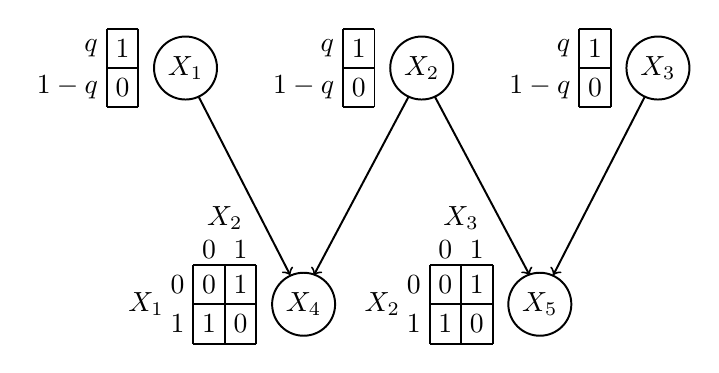
\begin{tikzpicture}

				\draw[line width = 0.25mm] (-3,3) circle (4mm);
				\node at (-3,3) {$X_1$};
				\draw[line width = 0.25mm] (0,3) circle (4mm);
				\node at (0,3) {$X_2$};
				\draw[line width = 0.25mm] (3,3) circle (4mm);
				\node at (3,3) {$X_3$};

				\draw[line width = 0.25mm] (-1.5,0) circle (4mm);
				\node at (-1.5,0) {$X_4$};
				\draw[line width = 0.25mm] (1.5,0) circle (4mm);
				\node at (1.5,0) {$X_5$};

				\draw[line width = 0.25mm][->] (-2.83,2.63) -- (-1.67,0.37);

				\draw[line width = 0.25mm][->] (-0.17,2.63) -- (-1.37,0.37);

				\draw[line width = 0.25mm][->] (0.17,2.63) -- (1.37,0.37);

				\draw[line width = 0.25mm][->] (2.83,2.63) -- (1.67,0.37);

				\draw[line width = 0.25mm] (-3.6,3) -- (-4,3);
				\draw[line width = 0.25mm] (-3.6,3.5) -- (-4,3.5);
				\draw[line width = 0.25mm] (-3.6,2.5) -- (-4,2.5);
				\draw[line width = 0.25mm] (-3.6,3.5) -- (-3.6,2.5);
				\draw[line width = 0.25mm] (-4,3.5) -- (-4,2.5);
				\node at (-3.8,3.25) {$1$};
				\node at (-3.8,2.75) {$0$};
				\node at (-4.2, 3.25) {$q$};
				\node at (-4.5, 2.75) {$1-q$};

				\draw[line width = 0.25mm] (-0.6,3) -- (-1,3);
				\draw[line width = 0.25mm] (-0.6,3.5) -- (-1,3.5);
				\draw[line width = 0.25mm] (-0.6,2.5) -- (-1,2.5);
				\draw[line width = 0.25mm] (-0.6,3.5) -- (-0.6,2.5);
				\draw[line width = 0.25mm] (-1,3.5) -- (-1,2.5);
				\node at (-0.8,3.25) {$1$};
				\node at (-0.8,2.75) {$0$};
				\node at (-1.2, 3.25) {$q$};
				\node at (-1.5, 2.75) {$1-q$};

				\draw[line width = 0.25mm] (2.4,3) -- (2,3);
				\draw[line width = 0.25mm] (2.4,3.5) -- (2,3.5);
				\draw[line width = 0.25mm] (2.4,2.5) -- (2,2.5);
				\draw[line width = 0.25mm] (2.4,3.5) -- (2.4,2.5);
				\draw[line width = 0.25mm] (2,3.5) -- (2,2.5);
				\node at (2.2,3.25) {$1$};
				\node at (2.2,2.75) {$0$};
				\node at (1.8, 3.25) {$q$};
				\node at (1.5, 2.75) {$1-q$};

				\draw[line width = 0.25mm] (-2.1,0) -- (-2.9,0);
				\draw[line width = 0.25mm] (-2.1,0.5) -- (-2.9,0.5);
				\draw[line width = 0.25mm] (-2.1,-0.5) -- (-2.9,-0.5);
				\draw[line width = 0.25mm] (-2.1,0.5) -- (-2.1,-0.5);
				\draw[line width = 0.25mm] (-2.9,0.5) -- (-2.9,-0.5);
				\draw[line width = 0.25mm] (-2.5,0.5) -- (-2.5,-0.5);
				\node at (-2.3,0.25) {$1$};
				\node at (-2.3,-0.25) {$0$};
				\node at (-2.7,0.25) {$0$};
				\node at (-2.7,-0.25) {$1$};

				\node at (-3.1, 0.25) {$0$};
				\node at (-3.1, -0.25) {$1$};
				\node at (-2.7, 0.7) {$0$};
				\node at (-2.3, 0.7) {$1$};

				\node at (-3.5, 0) {$X_1$};
				\node at (-2.5, 1.1) {$X_2$};

				\draw[line width = 0.25mm] (0.9,0) -- (0.1,0);
				\draw[line width = 0.25mm] (0.9,0.5) -- (0.1,0.5);
				\draw[line width = 0.25mm] (0.9,-0.5) -- (0.1,-0.5);
				\draw[line width = 0.25mm] (0.9,0.5) -- (0.9,-0.5);
				\draw[line width = 0.25mm] (0.1,0.5) -- (0.1,-0.5);
				\draw[line width = 0.25mm] (0.5,0.5) -- (0.5,-0.5);
				\node at (0.3,0.25) {$0$};
				\node at (0.3,-0.25) {$1$};
				\node at (0.7,0.25) {$1$};
				\node at (0.7,-0.25) {$0$};

				\node at (-0.1, 0.25) {$0$};
				\node at (-0.1, -0.25) {$1$};
				\node at (0.7, 0.7) {$1$};
				\node at (0.3, 0.7) {$0$};

				\node at (-0.5, 0) {$X_2$};
				\node at (0.5, 1.1) {$X_3$};

			\end{tikzpicture}
		\end{center}

		\bigbreak

		In order to determine at least five conditional independence relations from the directed graphical model, we apply Baye's Ball Theorem, in order to determine conditional independence of discrete random variables. To help with the construction of conditional independence relations, we will use the directed graphical models below.

		\bigbreak

		\begin{center}
			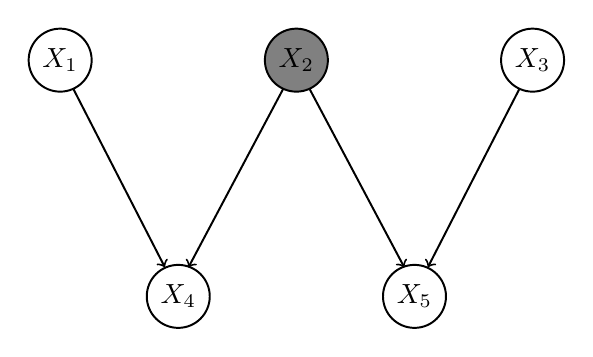
\begin{tikzpicture}

				\draw[line width = 0.25mm] (-3,3) circle (4mm);
				\node at (-3,3) {$X_1$};
				\draw[line width = 0.25mm][fill = gray] (0,3) circle (4mm);
				\node at (0,3) {$X_2$};
				\draw[line width = 0.25mm] (3,3) circle (4mm);
				\node at (3,3) {$X_3$};

				\draw[line width = 0.25mm] (-1.5,0) circle (4mm);
				\node at (-1.5,0) {$X_4$};
				\draw[line width = 0.25mm] (1.5,0) circle (4mm);
				\node at (1.5,0) {$X_5$};

				\draw[line width = 0.25mm][->] (-2.83,2.63) -- (-1.67,0.37);

				\draw[line width = 0.25mm][->] (-0.17,2.63) -- (-1.37,0.37);

				\draw[line width = 0.25mm][->] (0.17,2.63) -- (1.37,0.37);

				\draw[line width = 0.25mm][->] (2.83,2.63) -- (1.67,0.37);

			\end{tikzpicture}
		\end{center}

		\bigbreak

		Thus, it is clear that we have the following four conditional independence relations, derived from the rules that govern the behaviour the theoretical balls within Baye's Ball Theorem.

		\begin{enumerate}
			\item $\displaystyle{X_1 \indep X_5 | X_2}$
			\item $\displaystyle{X_1 \indep X_3 | X_2}$
			\item $\displaystyle{X_4 \indep X_5 | X_2}$
			\item $\displaystyle{X_4 \indep X_3 | X_2}$

		\end{enumerate}

		In order to get the fifth result, we use the following directed graphical model.

		\bigbreak

		\begin{center}
			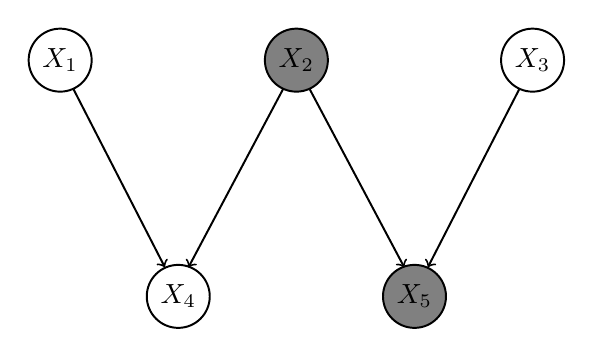
\begin{tikzpicture}

				\draw[line width = 0.25mm] (-3,3) circle (4mm);
				\node at (-3,3) {$X_1$};
				\draw[line width = 0.25mm][fill = gray] (0,3) circle (4mm);
				\node at (0,3) {$X_2$};
				\draw[line width = 0.25mm] (3,3) circle (4mm);
				\node at (3,3) {$X_3$};

				\draw[line width = 0.25mm] (-1.5,0) circle (4mm);
				\node at (-1.5,0) {$X_4$};
				\draw[line width = 0.25mm][fill = gray] (1.5,0) circle (4mm);
				\node at (1.5,0) {$X_5$};

				\draw[line width = 0.25mm][->] (-2.83,2.63) -- (-1.67,0.37);

				\draw[line width = 0.25mm][->] (-0.17,2.63) -- (-1.37,0.37);

				\draw[line width = 0.25mm][->] (0.17,2.63) -- (1.37,0.37);

				\draw[line width = 0.25mm][->] (2.83,2.63) -- (1.67,0.37);

			\end{tikzpicture}
		\end{center}

		\bigbreak

		Thus the fifth conditional independence relation is $\displaystyle{X_1 \indep X_3 | (X_2,X_5)}$. Thus, we have derived five conditional independence relations from the directed graphical model, utilising Baye's Ball Theorem and its governing laws.
		
		\bigbreak

		\item We are now required to determine the necessary conditions that exist upon $\displaystyle{q}$, in order to have $\displaystyle{X_3 \indep X_5}$, and $\displaystyle{X_1 \indep X_4}$. As we have $\displaystyle{X_3 \indep X_5}$ and $\displaystyle{X_1 \indep X_4}$, we are unable to apply Baye's Ball Theorem, as it is not conditional independence. Furthermore, independence in this example means that whatever the value that $\displaystyle{X_1}$ or $\displaystyle{X_3}$ takes has no influence on the value that $\displaystyle{X_4}$ or $\displaystyle{X_5}$ can take respectively. As a result, $\displaystyle{X_1}$ or $\displaystyle{X_3}$ must be able to take the values 0 and 1 with equal probability. Thus we have the following consequences.
		\begin{align*}
		q & = 1 - q \\
		\therefore 2q & = 1 \\
		\therefore q & = \frac{1}{2} \\
		\end{align*}
		These marginal independence assertions are not clear, nor implied from the graph in part (b).

	\end{enumerate}

	\bigbreak

	\item Consider the following directed graph.

	\bigbreak

	\begin{center}
		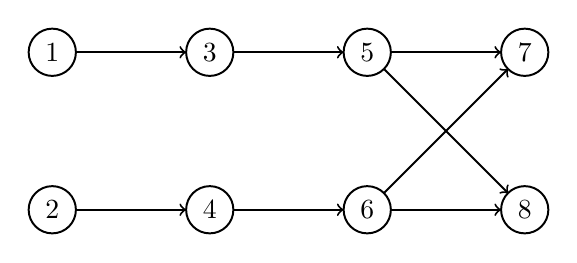
\begin{tikzpicture}

			\draw[line width = 0.25mm] (-3,2) circle (3mm);
			\node at (-3,2) {$1$};
			\draw[line width = 0.25mm] (-1,2) circle (3mm);
			\node at (-1,2) {$3$};
			\draw[line width = 0.25mm] (1,2) circle (3mm);
			\node at (1,2) {$5$};
			\draw[line width = 0.25mm] (3,2) circle (3mm);
			\node at (3,2) {$7$};

			\draw[line width = 0.25mm] (-3,0) circle (3mm);
			\node at (-3,0) {$2$};
			\draw[line width = 0.25mm] (-1,0) circle (3mm);
			\node at (-1,0) {$4$};
			\draw[line width = 0.25mm] (1,0) circle (3mm);
			\node at (1,0) {$6$};
			\draw[line width = 0.25mm] (3,0) circle (3mm);
			\node at (3,0) {$8$};

			\draw[line width = 0.25mm][->] (-2.70,2) -- (-1.3,2);
			\draw[line width = 0.25mm][->] (-0.70,2) -- (0.70,2);
			\draw[line width = 0.25mm][->] (1.3,2) -- (2.70,2);

			\draw[line width = 0.25mm][->] (-2.70,0) -- (-1.3,0);
			\draw[line width = 0.25mm][->] (-0.70,0) -- (0.70,0);
			\draw[line width = 0.25mm][->] (1.3,0) -- (2.70,0);

			\draw[line width = 0.25mm][->] (1.21,1.79) -- (2.79,0.21);
			\draw[line width = 0.25mm][->] (1.21,0.21) -- (2.79,1.79);

		\end{tikzpicture}
	\end{center}

	\bigbreak

	\begin{enumerate}

		\item From the directed graph above, we get the following moral graph.

		\bigbreak

		\begin{center}
			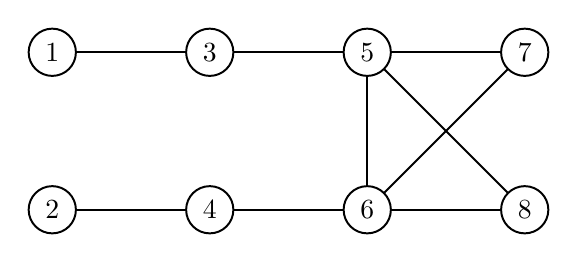
\begin{tikzpicture}

				\draw[line width = 0.25mm] (-3,2) circle (3mm);
				\node at (-3,2) {$1$};
				\draw[line width = 0.25mm] (-1,2) circle (3mm);
				\node at (-1,2) {$3$};
				\draw[line width = 0.25mm] (1,2) circle (3mm);
				\node at (1,2) {$5$};
				\draw[line width = 0.25mm] (3,2) circle (3mm);
				\node at (3,2) {$7$};

				\draw[line width = 0.25mm] (-3,0) circle (3mm);
				\node at (-3,0) {$2$};
				\draw[line width = 0.25mm] (-1,0) circle (3mm);
				\node at (-1,0) {$4$};
				\draw[line width = 0.25mm] (1,0) circle (3mm);
				\node at (1,0) {$6$};
				\draw[line width = 0.25mm] (3,0) circle (3mm);
				\node at (3,0) {$8$};

				\draw[line width = 0.25mm] (-2.70,2) -- (-1.3,2);
				\draw[line width = 0.25mm] (-0.70,2) -- (0.70,2);
				\draw[line width = 0.25mm] (1.3,2) -- (2.70,2);

				\draw[line width = 0.25mm] (-2.70,0) -- (-1.3,0);
				\draw[line width = 0.25mm] (-0.70,0) -- (0.70,0);
				\draw[line width = 0.25mm] (1.3,0) -- (2.70,0);

				\draw[line width = 0.25mm] (1.21,1.79) -- (2.79,0.21);
				\draw[line width = 0.25mm] (1.21,0.21) -- (2.79,1.79);
				\draw[line width = 0.25mm] (1,1.70) -- (1,0.30);

			\end{tikzpicture}
		\end{center}

		\pagebreak

		\item The following sequences provide the results from running the graph elimination algorithm in the given orders.

		\begin{enumerate}

			\item $\displaystyle{\{8,7,2,4,6,5,3,1\}}$

			\bigbreak

			\begin{center}
				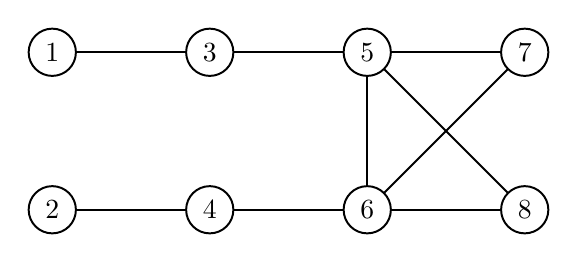
\begin{tikzpicture}

					\draw[line width = 0.25mm] (-3,2) circle (3mm);
					\node at (-3,2) {$1$};
					\draw[line width = 0.25mm] (-1,2) circle (3mm);
					\node at (-1,2) {$3$};
					\draw[line width = 0.25mm] (1,2) circle (3mm);
					\node at (1,2) {$5$};
					\draw[line width = 0.25mm] (3,2) circle (3mm);
					\node at (3,2) {$7$};

					\draw[line width = 0.25mm] (-3,0) circle (3mm);
					\node at (-3,0) {$2$};
					\draw[line width = 0.25mm] (-1,0) circle (3mm);
					\node at (-1,0) {$4$};
					\draw[line width = 0.25mm] (1,0) circle (3mm);
					\node at (1,0) {$6$};
					\draw[line width = 0.25mm] (3,0) circle (3mm);
					\node at (3,0) {$8$};

					\draw[line width = 0.25mm] (-2.70,2) -- (-1.3,2);
					\draw[line width = 0.25mm] (-0.70,2) -- (0.70,2);
					\draw[line width = 0.25mm] (1.3,2) -- (2.70,2);

					\draw[line width = 0.25mm] (-2.70,0) -- (-1.3,0);
					\draw[line width = 0.25mm] (-0.70,0) -- (0.70,0);
					\draw[line width = 0.25mm] (1.3,0) -- (2.70,0);

					\draw[line width = 0.25mm] (1.21,1.79) -- (2.79,0.21);
					\draw[line width = 0.25mm] (1.21,0.21) -- (2.79,1.79);
					\draw[line width = 0.25mm] (1,1.70) -- (1,0.30);

				\end{tikzpicture}
			\end{center}

			\bigbreak

			\begin{center}
				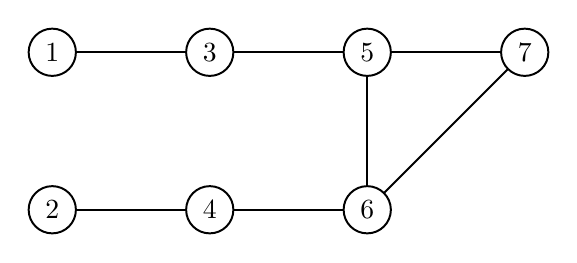
\begin{tikzpicture}

					\draw[line width = 0.25mm] (-3,2) circle (3mm);
					\node at (-3,2) {$1$};
					\draw[line width = 0.25mm] (-1,2) circle (3mm);
					\node at (-1,2) {$3$};
					\draw[line width = 0.25mm] (1,2) circle (3mm);
					\node at (1,2) {$5$};
					\draw[line width = 0.25mm] (3,2) circle (3mm);
					\node at (3,2) {$7$};

					\draw[line width = 0.25mm] (-3,0) circle (3mm);
					\node at (-3,0) {$2$};
					\draw[line width = 0.25mm] (-1,0) circle (3mm);
					\node at (-1,0) {$4$};
					\draw[line width = 0.25mm] (1,0) circle (3mm);
					\node at (1,0) {$6$};

					\draw[line width = 0.25mm] (-2.70,2) -- (-1.3,2);
					\draw[line width = 0.25mm] (-0.70,2) -- (0.70,2);
					\draw[line width = 0.25mm] (1.3,2) -- (2.70,2);

					\draw[line width = 0.25mm] (-2.70,0) -- (-1.3,0);
					\draw[line width = 0.25mm] (-0.70,0) -- (0.70,0);


					\draw[line width = 0.25mm] (1.21,0.21) -- (2.79,1.79);
					\draw[line width = 0.25mm] (1,1.70) -- (1,0.30);

				\end{tikzpicture}
			\end{center}

			\bigbreak

			\begin{center}
				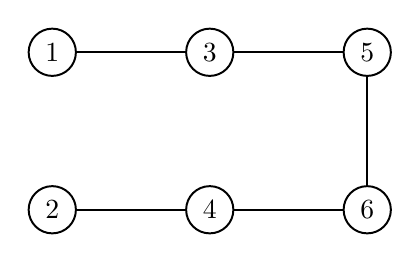
\begin{tikzpicture}

					\draw[line width = 0.25mm] (-3,2) circle (3mm);
					\node at (-3,2) {$1$};
					\draw[line width = 0.25mm] (-1,2) circle (3mm);
					\node at (-1,2) {$3$};
					\draw[line width = 0.25mm] (1,2) circle (3mm);
					\node at (1,2) {$5$};

					\draw[line width = 0.25mm] (-3,0) circle (3mm);
					\node at (-3,0) {$2$};
					\draw[line width = 0.25mm] (-1,0) circle (3mm);
					\node at (-1,0) {$4$};
					\draw[line width = 0.25mm] (1,0) circle (3mm);
					\node at (1,0) {$6$};

					\draw[line width = 0.25mm] (-2.70,2) -- (-1.3,2);
					\draw[line width = 0.25mm] (-0.70,2) -- (0.70,2);

					\draw[line width = 0.25mm] (-2.70,0) -- (-1.3,0);
					\draw[line width = 0.25mm] (-0.70,0) -- (0.70,0);

					\draw[line width = 0.25mm] (1,1.70) -- (1,0.30);

				\end{tikzpicture}
			\end{center}

			\bigbreak

			\begin{center}
				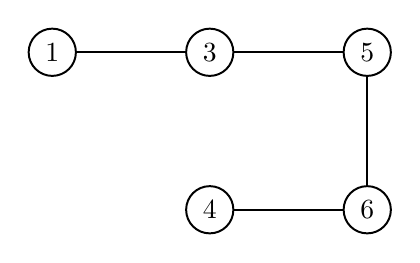
\begin{tikzpicture}

					\draw[line width = 0.25mm] (-3,2) circle (3mm);
					\node at (-3,2) {$1$};
					\draw[line width = 0.25mm] (-1,2) circle (3mm);
					\node at (-1,2) {$3$};
					\draw[line width = 0.25mm] (1,2) circle (3mm);
					\node at (1,2) {$5$};

					\draw[line width = 0.25mm] (-1,0) circle (3mm);
					\node at (-1,0) {$4$};
					\draw[line width = 0.25mm] (1,0) circle (3mm);
					\node at (1,0) {$6$};

					\draw[line width = 0.25mm] (-2.70,2) -- (-1.3,2);
					\draw[line width = 0.25mm] (-0.70,2) -- (0.70,2);

					\draw[line width = 0.25mm] (-0.70,0) -- (0.70,0);

					\draw[line width = 0.25mm] (1,1.70) -- (1,0.30);

				\end{tikzpicture}
			\end{center}

			\bigbreak

			\begin{center}
				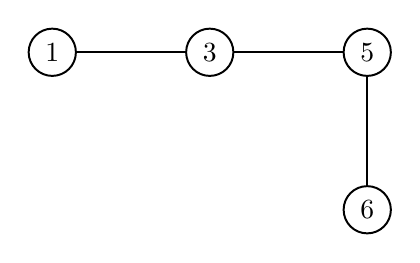
\begin{tikzpicture}

					\draw[line width = 0.25mm] (-3,2) circle (3mm);
					\node at (-3,2) {$1$};
					\draw[line width = 0.25mm] (-1,2) circle (3mm);
					\node at (-1,2) {$3$};
					\draw[line width = 0.25mm] (1,2) circle (3mm);
					\node at (1,2) {$5$};

					\draw[line width = 0.25mm] (1,0) circle (3mm);
					\node at (1,0) {$6$};

					\draw[line width = 0.25mm] (-2.70,2) -- (-1.3,2);
					\draw[line width = 0.25mm] (-0.70,2) -- (0.70,2);

					\draw[line width = 0.25mm] (1,1.70) -- (1,0.30);

				\end{tikzpicture}
			\end{center}

			\bigbreak

			\begin{center}
				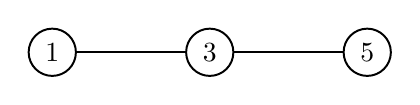
\begin{tikzpicture}

					\draw[line width = 0.25mm] (-3,2) circle (3mm);
					\node at (-3,2) {$1$};
					\draw[line width = 0.25mm] (-1,2) circle (3mm);
					\node at (-1,2) {$3$};
					\draw[line width = 0.25mm] (1,2) circle (3mm);
					\node at (1,2) {$5$};

					\draw[line width = 0.25mm] (-2.70,2) -- (-1.3,2);
					\draw[line width = 0.25mm] (-0.70,2) -- (0.70,2);

				\end{tikzpicture}
			\end{center}

			\bigbreak

			\begin{center}
				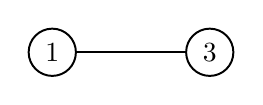
\begin{tikzpicture}

					\draw[line width = 0.25mm] (-3,2) circle (3mm);
					\node at (-3,2) {$1$};
					\draw[line width = 0.25mm] (-1,2) circle (3mm);
					\node at (-1,2) {$3$};

					\draw[line width = 0.25mm] (-2.70,2) -- (-1.3,2);

				\end{tikzpicture}
			\end{center}

			\bigbreak

			\begin{center}
				
\begin{tikzpicture}

					\draw[line width = 0.25mm] (-3,2) circle (3mm);
					\node at (-3,2) {$1$};

				\end{tikzpicture}
			\end{center}

			\pagebreak

			\item $\displaystyle{\{8,5,6,7,4,3,2,1\}}$

			\begin{center}
				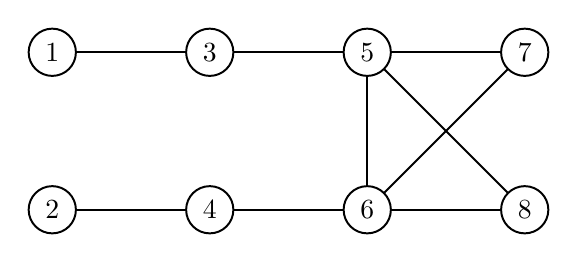
\begin{tikzpicture}

					\draw[line width = 0.25mm] (-3,2) circle (3mm);
					\node at (-3,2) {$1$};
					\draw[line width = 0.25mm] (-1,2) circle (3mm);
					\node at (-1,2) {$3$};
					\draw[line width = 0.25mm] (1,2) circle (3mm);
					\node at (1,2) {$5$};
					\draw[line width = 0.25mm] (3,2) circle (3mm);
					\node at (3,2) {$7$};

					\draw[line width = 0.25mm] (-3,0) circle (3mm);
					\node at (-3,0) {$2$};
					\draw[line width = 0.25mm] (-1,0) circle (3mm);
					\node at (-1,0) {$4$};
					\draw[line width = 0.25mm] (1,0) circle (3mm);
					\node at (1,0) {$6$};
					\draw[line width = 0.25mm] (3,0) circle (3mm);
					\node at (3,0) {$8$};

					\draw[line width = 0.25mm] (-2.70,2) -- (-1.3,2);
					\draw[line width = 0.25mm] (-0.70,2) -- (0.70,2);
					\draw[line width = 0.25mm] (1.3,2) -- (2.70,2);

					\draw[line width = 0.25mm] (-2.70,0) -- (-1.3,0);
					\draw[line width = 0.25mm] (-0.70,0) -- (0.70,0);
					\draw[line width = 0.25mm] (1.3,0) -- (2.70,0);

					\draw[line width = 0.25mm] (1.21,1.79) -- (2.79,0.21);
					\draw[line width = 0.25mm] (1.21,0.21) -- (2.79,1.79);
					\draw[line width = 0.25mm] (1,1.70) -- (1,0.30);

				\end{tikzpicture}
			\end{center}

			\bigbreak

			\begin{center}
				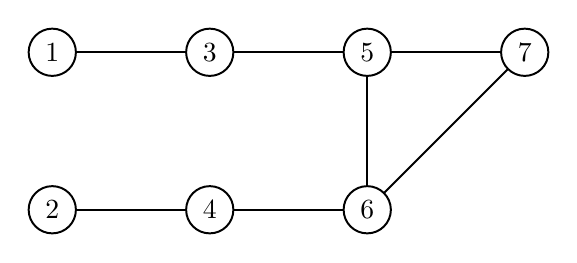
\begin{tikzpicture}

					\draw[line width = 0.25mm] (-3,2) circle (3mm);
					\node at (-3,2) {$1$};
					\draw[line width = 0.25mm] (-1,2) circle (3mm);
					\node at (-1,2) {$3$};
					\draw[line width = 0.25mm] (1,2) circle (3mm);
					\node at (1,2) {$5$};
					\draw[line width = 0.25mm] (3,2) circle (3mm);
					\node at (3,2) {$7$};

					\draw[line width = 0.25mm] (-3,0) circle (3mm);
					\node at (-3,0) {$2$};
					\draw[line width = 0.25mm] (-1,0) circle (3mm);
					\node at (-1,0) {$4$};
					\draw[line width = 0.25mm] (1,0) circle (3mm);
					\node at (1,0) {$6$};

					\draw[line width = 0.25mm] (-2.70,2) -- (-1.3,2);
					\draw[line width = 0.25mm] (-0.70,2) -- (0.70,2);
					\draw[line width = 0.25mm] (1.3,2) -- (2.70,2);

					\draw[line width = 0.25mm] (-2.70,0) -- (-1.3,0);
					\draw[line width = 0.25mm] (-0.70,0) -- (0.70,0);


					\draw[line width = 0.25mm] (1.21,0.21) -- (2.79,1.79);
					\draw[line width = 0.25mm] (1,1.70) -- (1,0.30);

				\end{tikzpicture}
			\end{center}

			\bigbreak

			\begin{center}
				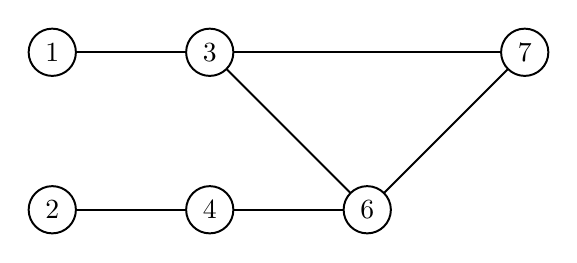
\begin{tikzpicture}

					\draw[line width = 0.25mm] (-3,2) circle (3mm);
					\node at (-3,2) {$1$};
					\draw[line width = 0.25mm] (-1,2) circle (3mm);
					\node at (-1,2) {$3$};
					\draw[line width = 0.25mm] (3,2) circle (3mm);
					\node at (3,2) {$7$};

					\draw[line width = 0.25mm] (-3,0) circle (3mm);
					\node at (-3,0) {$2$};
					\draw[line width = 0.25mm] (-1,0) circle (3mm);
					\node at (-1,0) {$4$};
					\draw[line width = 0.25mm] (1,0) circle (3mm);
					\node at (1,0) {$6$};

					\draw[line width = 0.25mm] (-2.70,2) -- (-1.3,2);
					\draw[line width = 0.25mm] (-0.70,2) -- (2.70,2);

					\draw[line width = 0.25mm] (-2.70,0) -- (-1.3,0);
					\draw[line width = 0.25mm] (-0.70,0) -- (0.70,0);

					\draw[line width = 0.25mm] (1.21,0.21) -- (2.79,1.79);
					\draw[line width = 0.25mm] (0.79,0.21) -- (-0.79,1.79);

				\end{tikzpicture}
			\end{center}

			\bigbreak

			\begin{center}
				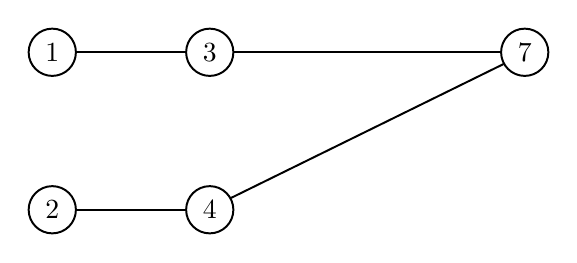
\begin{tikzpicture}

					\draw[line width = 0.25mm] (-3,2) circle (3mm);
					\node at (-3,2) {$1$};
					\draw[line width = 0.25mm] (-1,2) circle (3mm);
					\node at (-1,2) {$3$};
					\draw[line width = 0.25mm] (3,2) circle (3mm);
					\node at (3,2) {$7$};

					\draw[line width = 0.25mm] (-3,0) circle (3mm);
					\node at (-3,0) {$2$};
					\draw[line width = 0.25mm] (-1,0) circle (3mm);
					\node at (-1,0) {$4$};

					\draw[line width = 0.25mm] (-2.70,2) -- (-1.3,2);
					\draw[line width = 0.25mm] (-0.70,2) -- (2.70,2);

					\draw[line width = 0.25mm] (-2.70,0) -- (-1.3,0);

					\draw[line width = 0.25mm] (-0.73,0.15) -- (2.73,1.85);

				\end{tikzpicture}
			\end{center}

			\bigbreak

			\begin{center}
				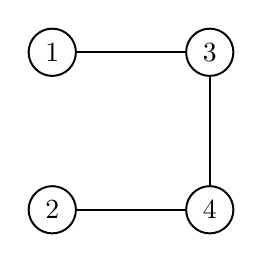
\begin{tikzpicture}

					\draw[line width = 0.25mm] (-3,2) circle (3mm);
					\node at (-3,2) {$1$};
					\draw[line width = 0.25mm] (-1,2) circle (3mm);
					\node at (-1,2) {$3$};

					\draw[line width = 0.25mm] (-3,0) circle (3mm);
					\node at (-3,0) {$2$};
					\draw[line width = 0.25mm] (-1,0) circle (3mm);
					\node at (-1,0) {$4$};

					\draw[line width = 0.25mm] (-2.70,2) -- (-1.3,2);

					\draw[line width = 0.25mm] (-2.70,0) -- (-1.3,0);

					\draw[line width = 0.25mm] (-1,1.70) -- (-1,0.30);


				\end{tikzpicture}
			\end{center}

			\bigbreak

			\begin{center}
				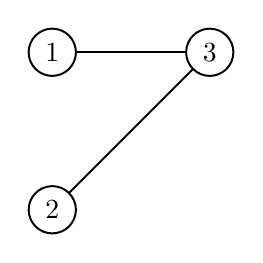
\begin{tikzpicture}

					\draw[line width = 0.25mm] (-3,2) circle (3mm);
					\node at (-3,2) {$1$};
					\draw[line width = 0.25mm] (-1,2) circle (3mm);
					\node at (-1,2) {$3$};

					\draw[line width = 0.25mm] (-3,0) circle (3mm);
					\node at (-3,0) {$2$};

					\draw[line width = 0.25mm] (-2.70,2) -- (-1.3,2);

					\draw[line width = 0.25mm] (-2.79,0.21) -- (-1.21,1.79);

				\end{tikzpicture}
			\end{center}

			\bigbreak

			\begin{center}
				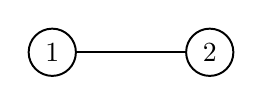
\begin{tikzpicture}

					\draw[line width = 0.25mm] (-3,2) circle (3mm);
					\node at (-3,2) {$1$};

					\draw[line width = 0.25mm] (-1,2) circle (3mm);
					\node at (-1,2) {$2$};

					\draw[line width = 0.25mm] (-2.70,2) -- (-1.3,2);

				\end{tikzpicture}
			\end{center}

			\bigbreak

			\begin{center}
				
\begin{tikzpicture}

					\draw[line width = 0.25mm] (-3,2) circle (3mm);
					\node at (-3,2) {$1$};

				\end{tikzpicture}
			\end{center}

		\end{enumerate}

		\bigbreak

		\item The first order used in the graph elimination algorithm, that is the order $\displaystyle{\{8,7,2,4,6,5,3,1\}}$ , is the best order for computing $\displaystyle{p(x_1|x_8)}$. This is because of the sequence of elimination, that does not add any connections between nodes that did not already exist, rather only removes them from the moral graph. However, using the second order does add connections that did not already exist on the moral graph, and thus is less preferable than the first.

	\end{enumerate}

	


\end{enumerate}





\end{document}